\documentclass[10pt]{beamer}

\usetheme[progressbar=foot, background=dark]{metropolis}
\usepackage{appendixnumberbeamer}

% fsts
\usepackage{tikz}
% strikethrough
\usepackage[normalem]{ulem}
% code listing thing
\usepackage{listings}


\usepackage{booktabs}
\usepackage[scale=2]{ccicons}

\usepackage{pgfplots}
\usepgfplotslibrary{dateplot}

\usepackage{subfigure}
\usepackage{gb4e}

\usepackage{xspace}
\newcommand{\themename}{\textbf{\textsc{metropolis}}\xspace}
\graphicspath{{figs/}}

\title{Things* I wish I knew* before starting a real job}
\subtitle{TODO:explain *}
\date{February 23, 2018}
\author{Trevor Sullivan}
% \institute{University of Arizona}
% \titlegraphic{\hfill\includegraphics[height=1.5cm]{logo.pdf}}

\begin{document}

\maketitle

\begin{frame}{Background in 30 seconds, GO!}
\pause
    \begin{itemize}[<+->]
    	\item Came to UofAZ as a music/linguistics student
    	\item Realized music is a dumb thing to spend \$40,000 on
    	\item Hey computers are cool
    	\item Double major in linguistics/CS
    	\item Masters program? hell yeah!
    	\item Internship with ayfie on fuzzy prefix search
    	\item Job?
    	\item yes
    	\item search for lawyers
    \end{itemize}
\pause
TIME

\end{frame}

\begin{frame}{Overview}
\pause
\begin{itemize}[<+->]
	\item I worked as an intern for ayfie for my hlt project on fuzzy prefix search
	(cf October 2016 Data Science Meetup)
	\item I was hired afterwards as a Professional Service Engineer, to start in May
	\item I took some notes on things* that I found particularly frustrating to not know* ahead of time
\end{itemize}
\pause
Starting any new job comes with a learning phase that lasts weeks or months, but knowing* about some things* ahead of time will help you make the transition more easily

\end{frame}

\begin{frame}
	\frametitle{On things and knowing}

	\begin{itemize}[<+->]
		\item Things
		\begin{itemize}[<+->]
			\item This is just an excuse for me to bring up \alert{impostor syndrome} because it didn't fit anywhere else in the talk
			\item it never goes away
			\item \textbf{NOW} is the time to practice your confidence and self esteem
		\end{itemize}
		\item Learning
		\begin{itemize}[<+->]
			\item learning \textit{about}
			\item \textit{learning} learning
		\end{itemize}
	\end{itemize}
\end{frame}


\begin{frame}{Table of contents}
  \setbeamertemplate{section in toc}[sections numbered]
  \tableofcontents[hideallsubsections]
\end{frame}



\section{System Administration | The Command Line}


\begin{frame}[c]
	\frametitle{Be aware of: Finer points of sysadmin}
	\pause
	When you're working on a server. you will need to learn some particular skills and methods to manage things

	\begin{description}[<+->]
		\item[Managing volumes] \texttt{df -h}, \texttt{fdisk}, \texttt{mkfs}
		\item[ssh tunnels and UDP] \texttt{ssh -L 18080:127.0.0.1:18085 -R 18086:127.0.0.1:18086 user@server}
		\item[web access control]  \texttt{nginx}
	\end{description}
\end{frame}


\begin{frame}[c]
	\frametitle{Do it now: The Command Line}
	\begin{itemize}[<+->]
		\item Navigating a *nix filesystem
		\item text editor (vim, emacs, nano)
		\item tmux or screen

		They may seem dumb at first, but you will soon find you can't live without it

		Like browsing without tabs
	\end{itemize}
\end{frame}

\begin{frame}[standout]
	\frametitle{tmux}

	\centerline{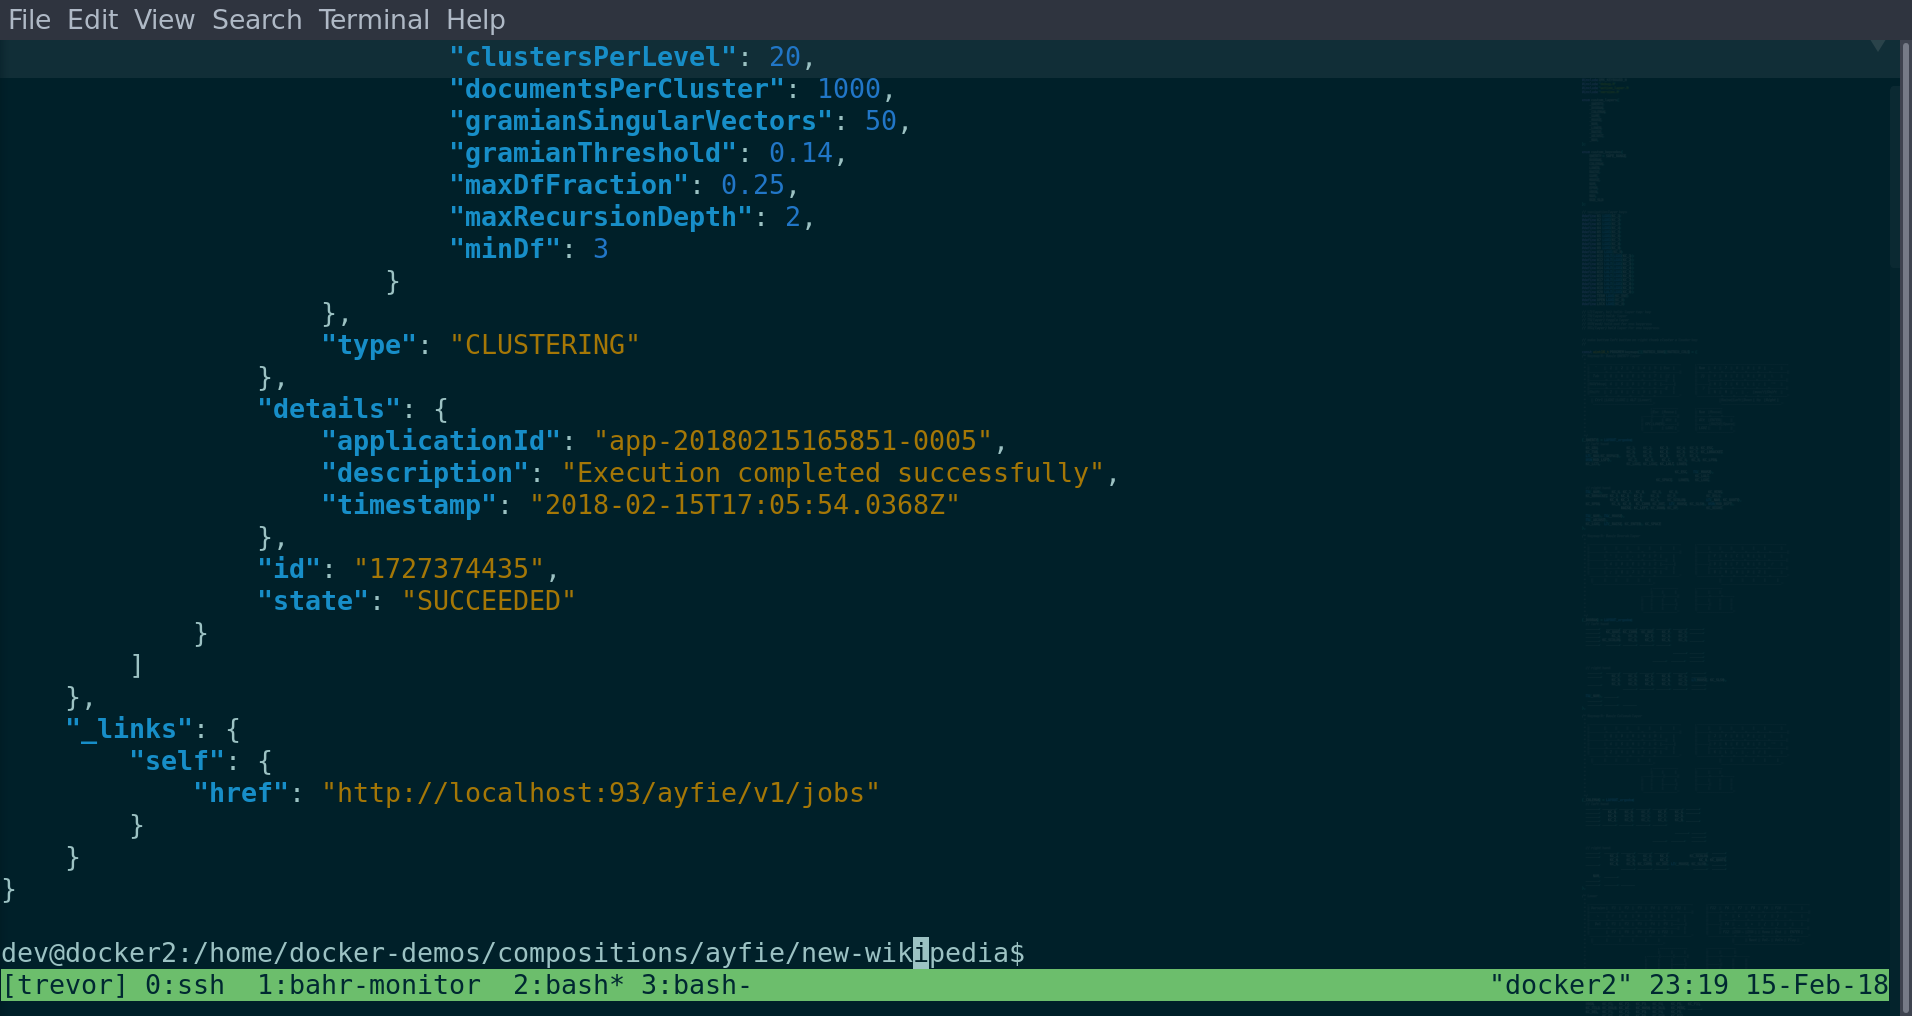
\includegraphics[width=12cm]{tmux.png}}
\end{frame}








\section{Team workflows | Personal task management}

\begin{frame}[c]
	\frametitle{Be aware of: Scrum and Team Workflows}
	\begin{itemize}[<+->]
		\item Every company does this a different way
		\item scrum master
		\item sprint review
		\item board
	\end{itemize}
\end{frame}

\begin{frame}[c]{Boards}
    \centerline{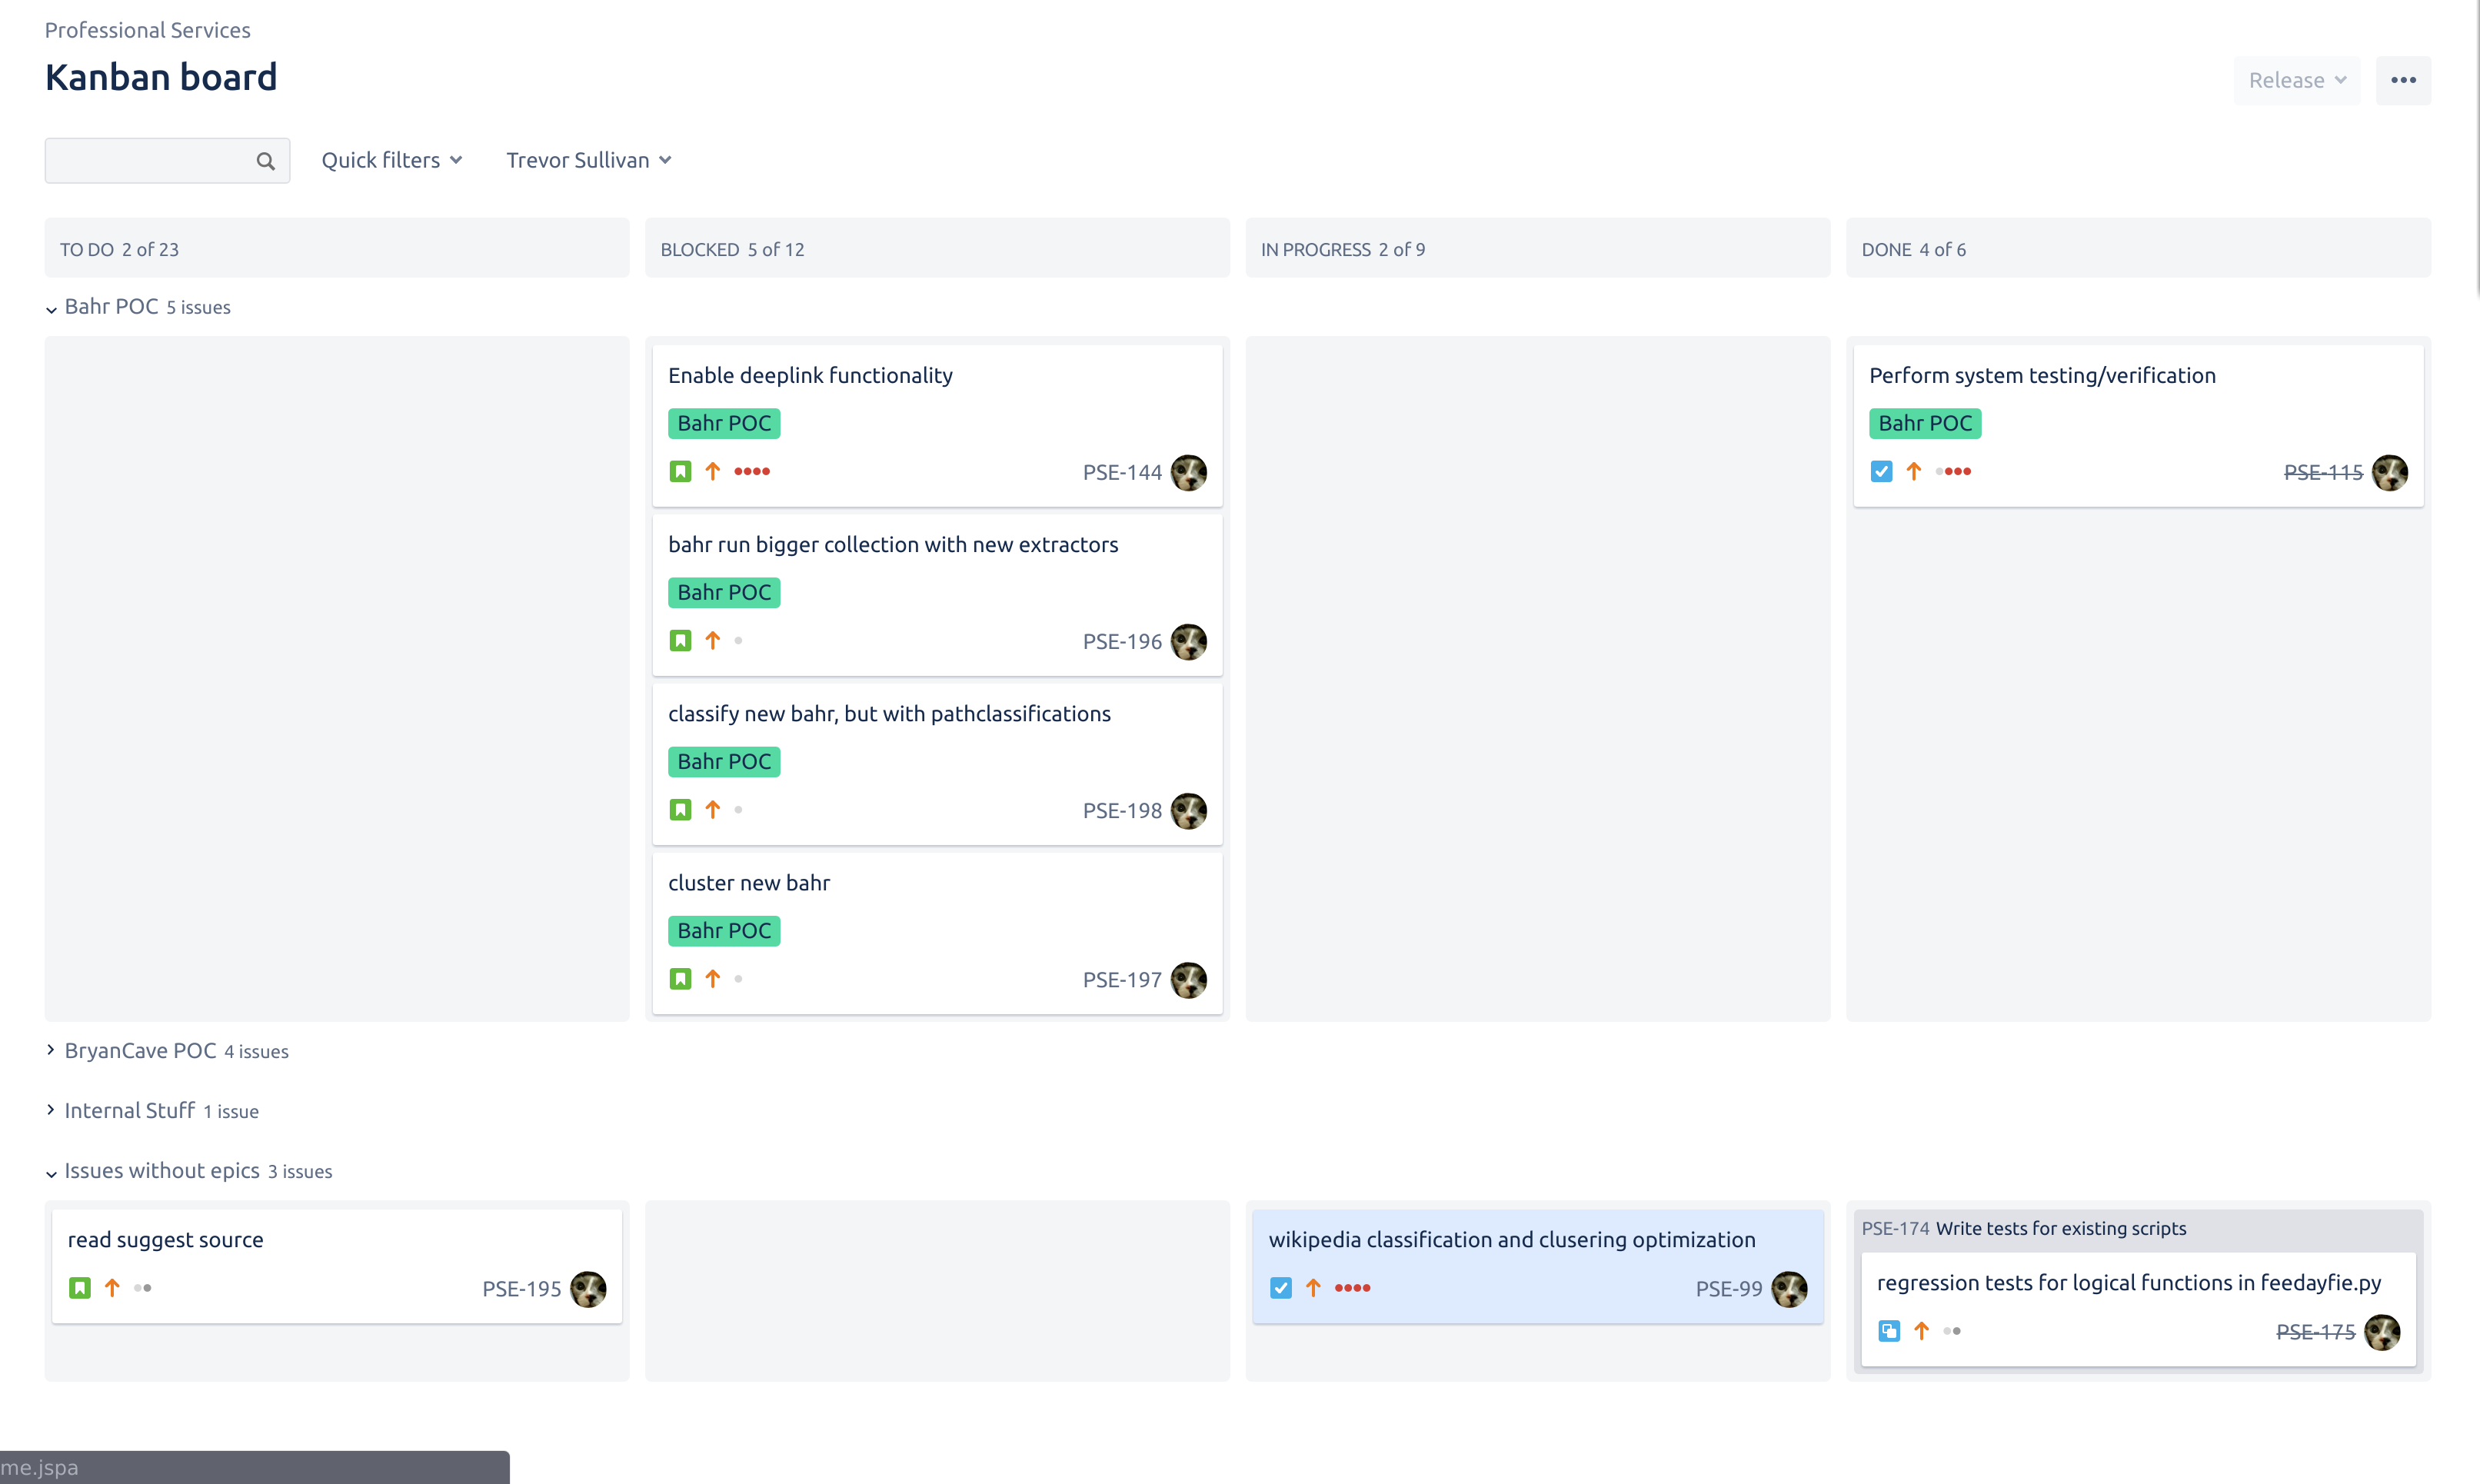
\includegraphics[width=10cm]{figs/pseboard.png}}


\end{frame}

\begin{frame}[c]{Boards}
    \centerline{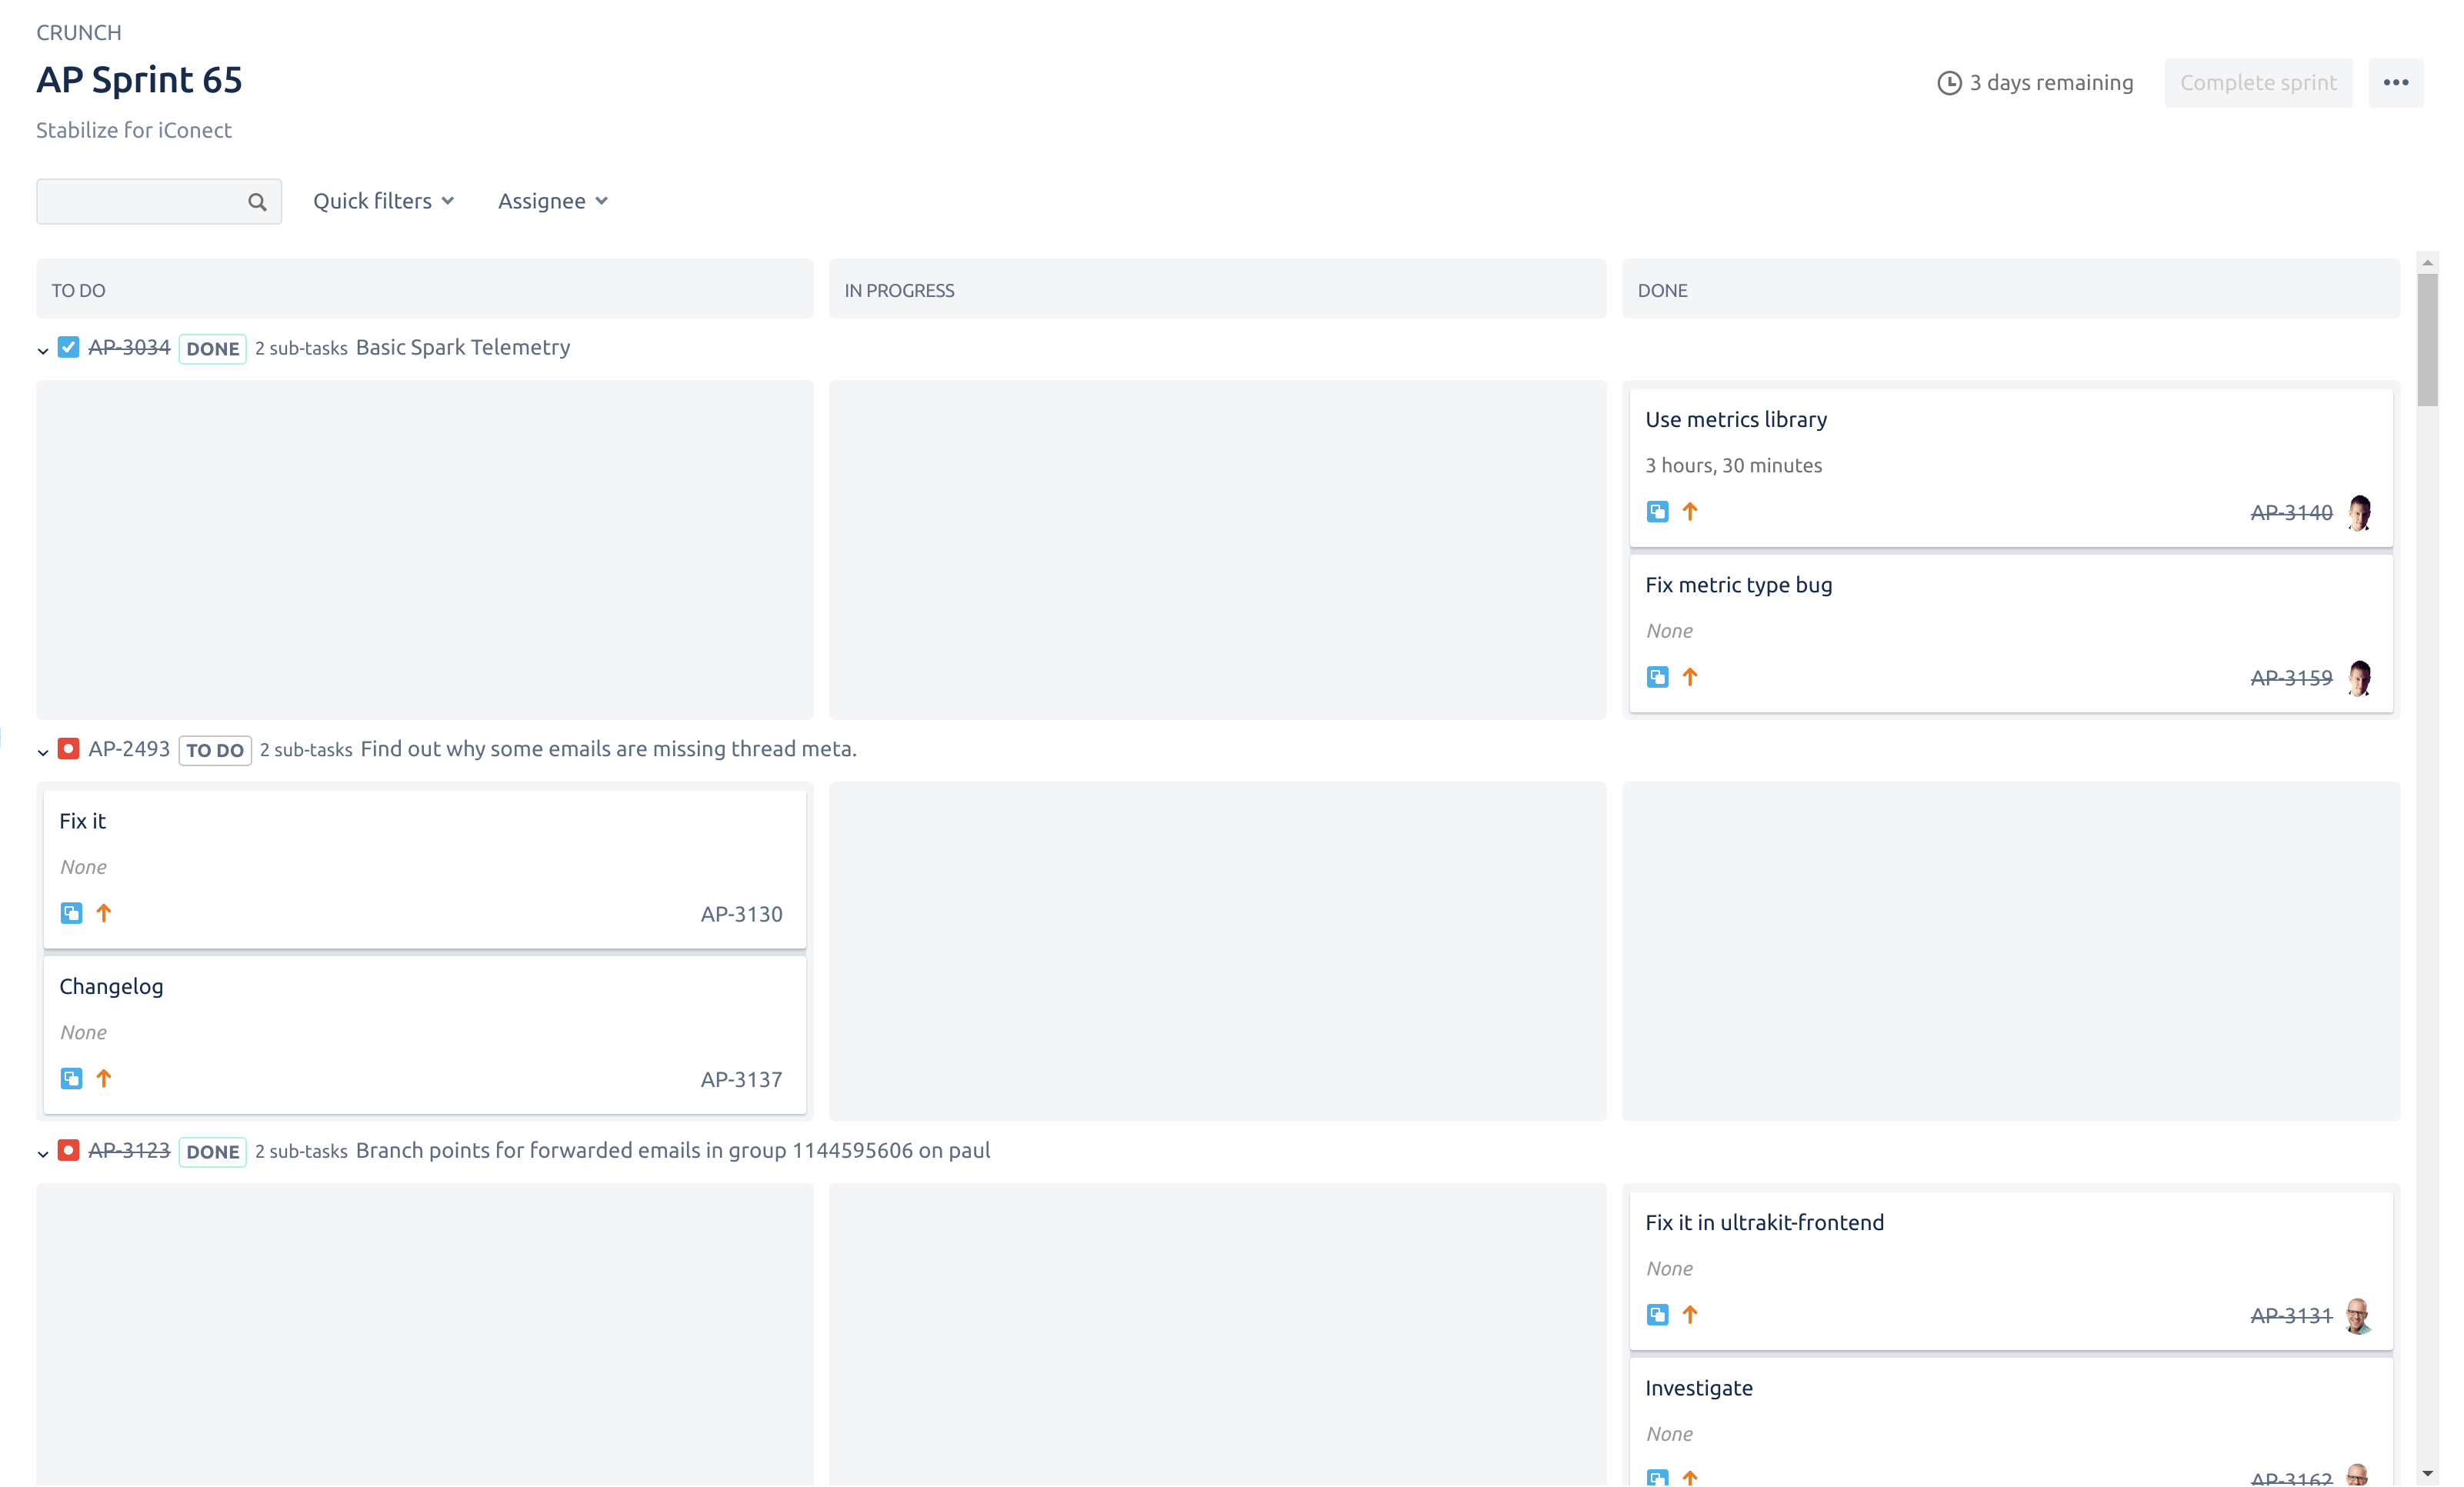
\includegraphics[width=10cm]{figs/apboard.png}}

\end{frame}

\begin{frame}[c]{Do it now: Task Management}
    \begin{itemize}[<+->]
    	\item People tend to overestimate their own ability to remember things
    	\item There is a limited amount of space in your working memory, and to commit something to long term memory, you need to call it back to working memory several times
    	\item This is a waste of brain power. Everything you have to remember distracts you.
    	\item Strive therefore to get things out of your head as soon as possible

    \end{itemize}


\end{frame}

\begin{frame}[c]{Apps: Asana}

\centerline{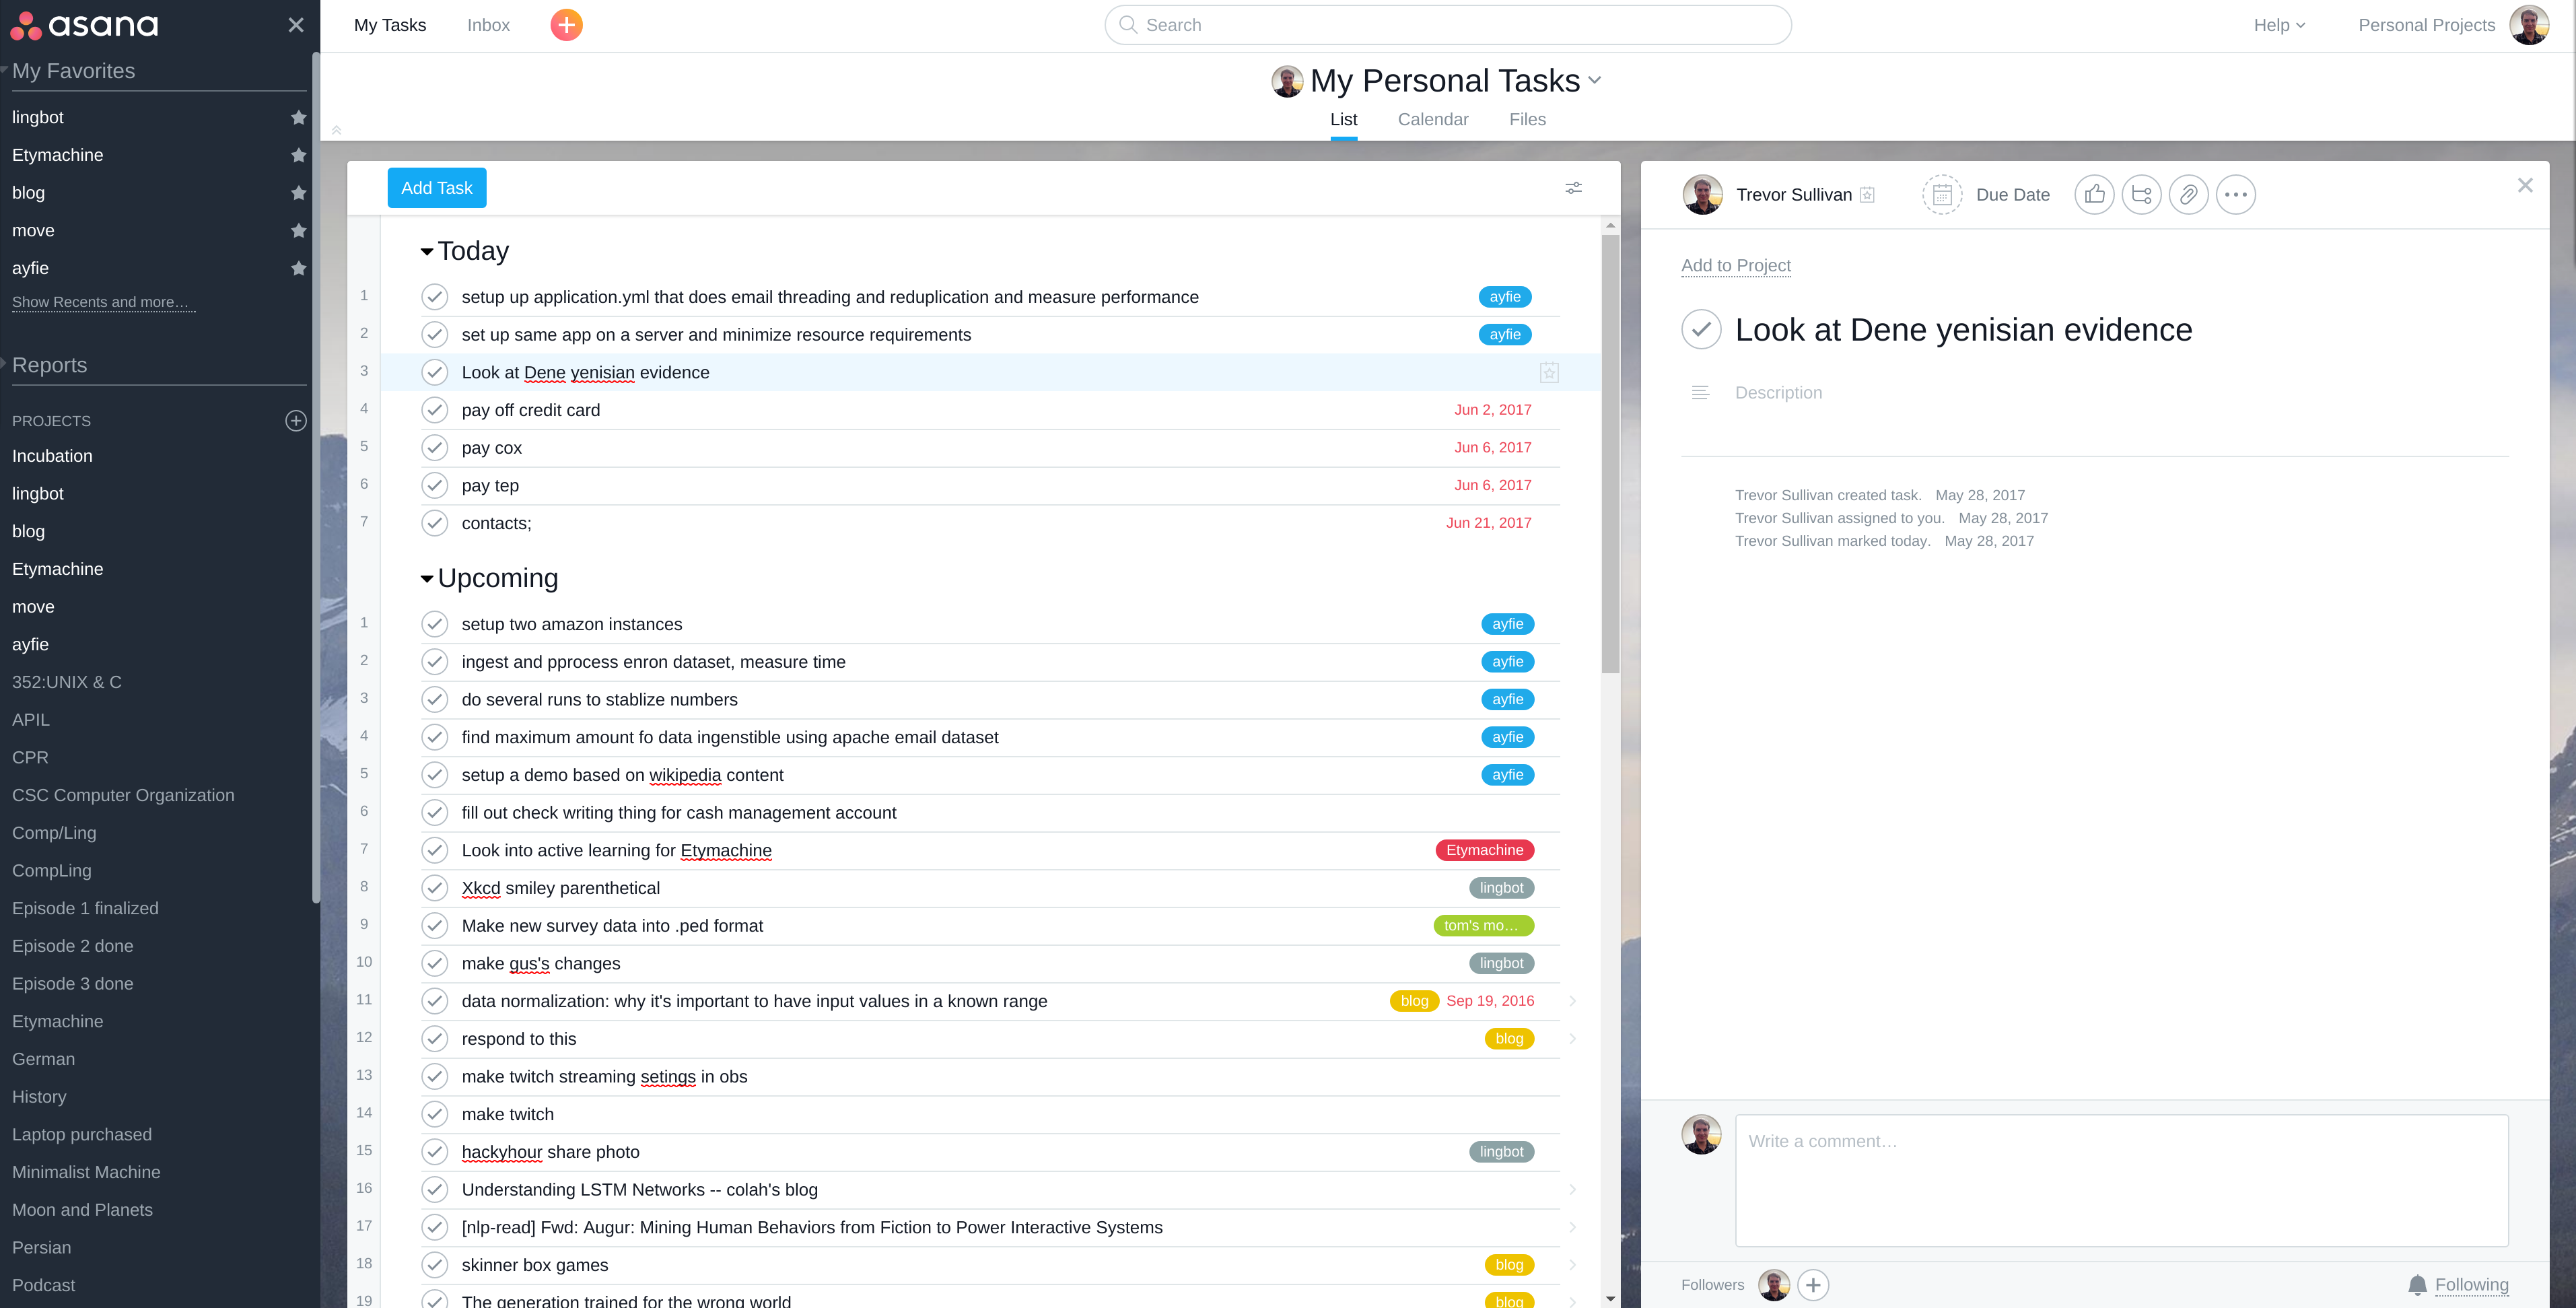
\includegraphics[width=12cm]{figs/asana.png}}

\end{frame}

\begin{frame}[c]{Apps: Todoist}

\centerline{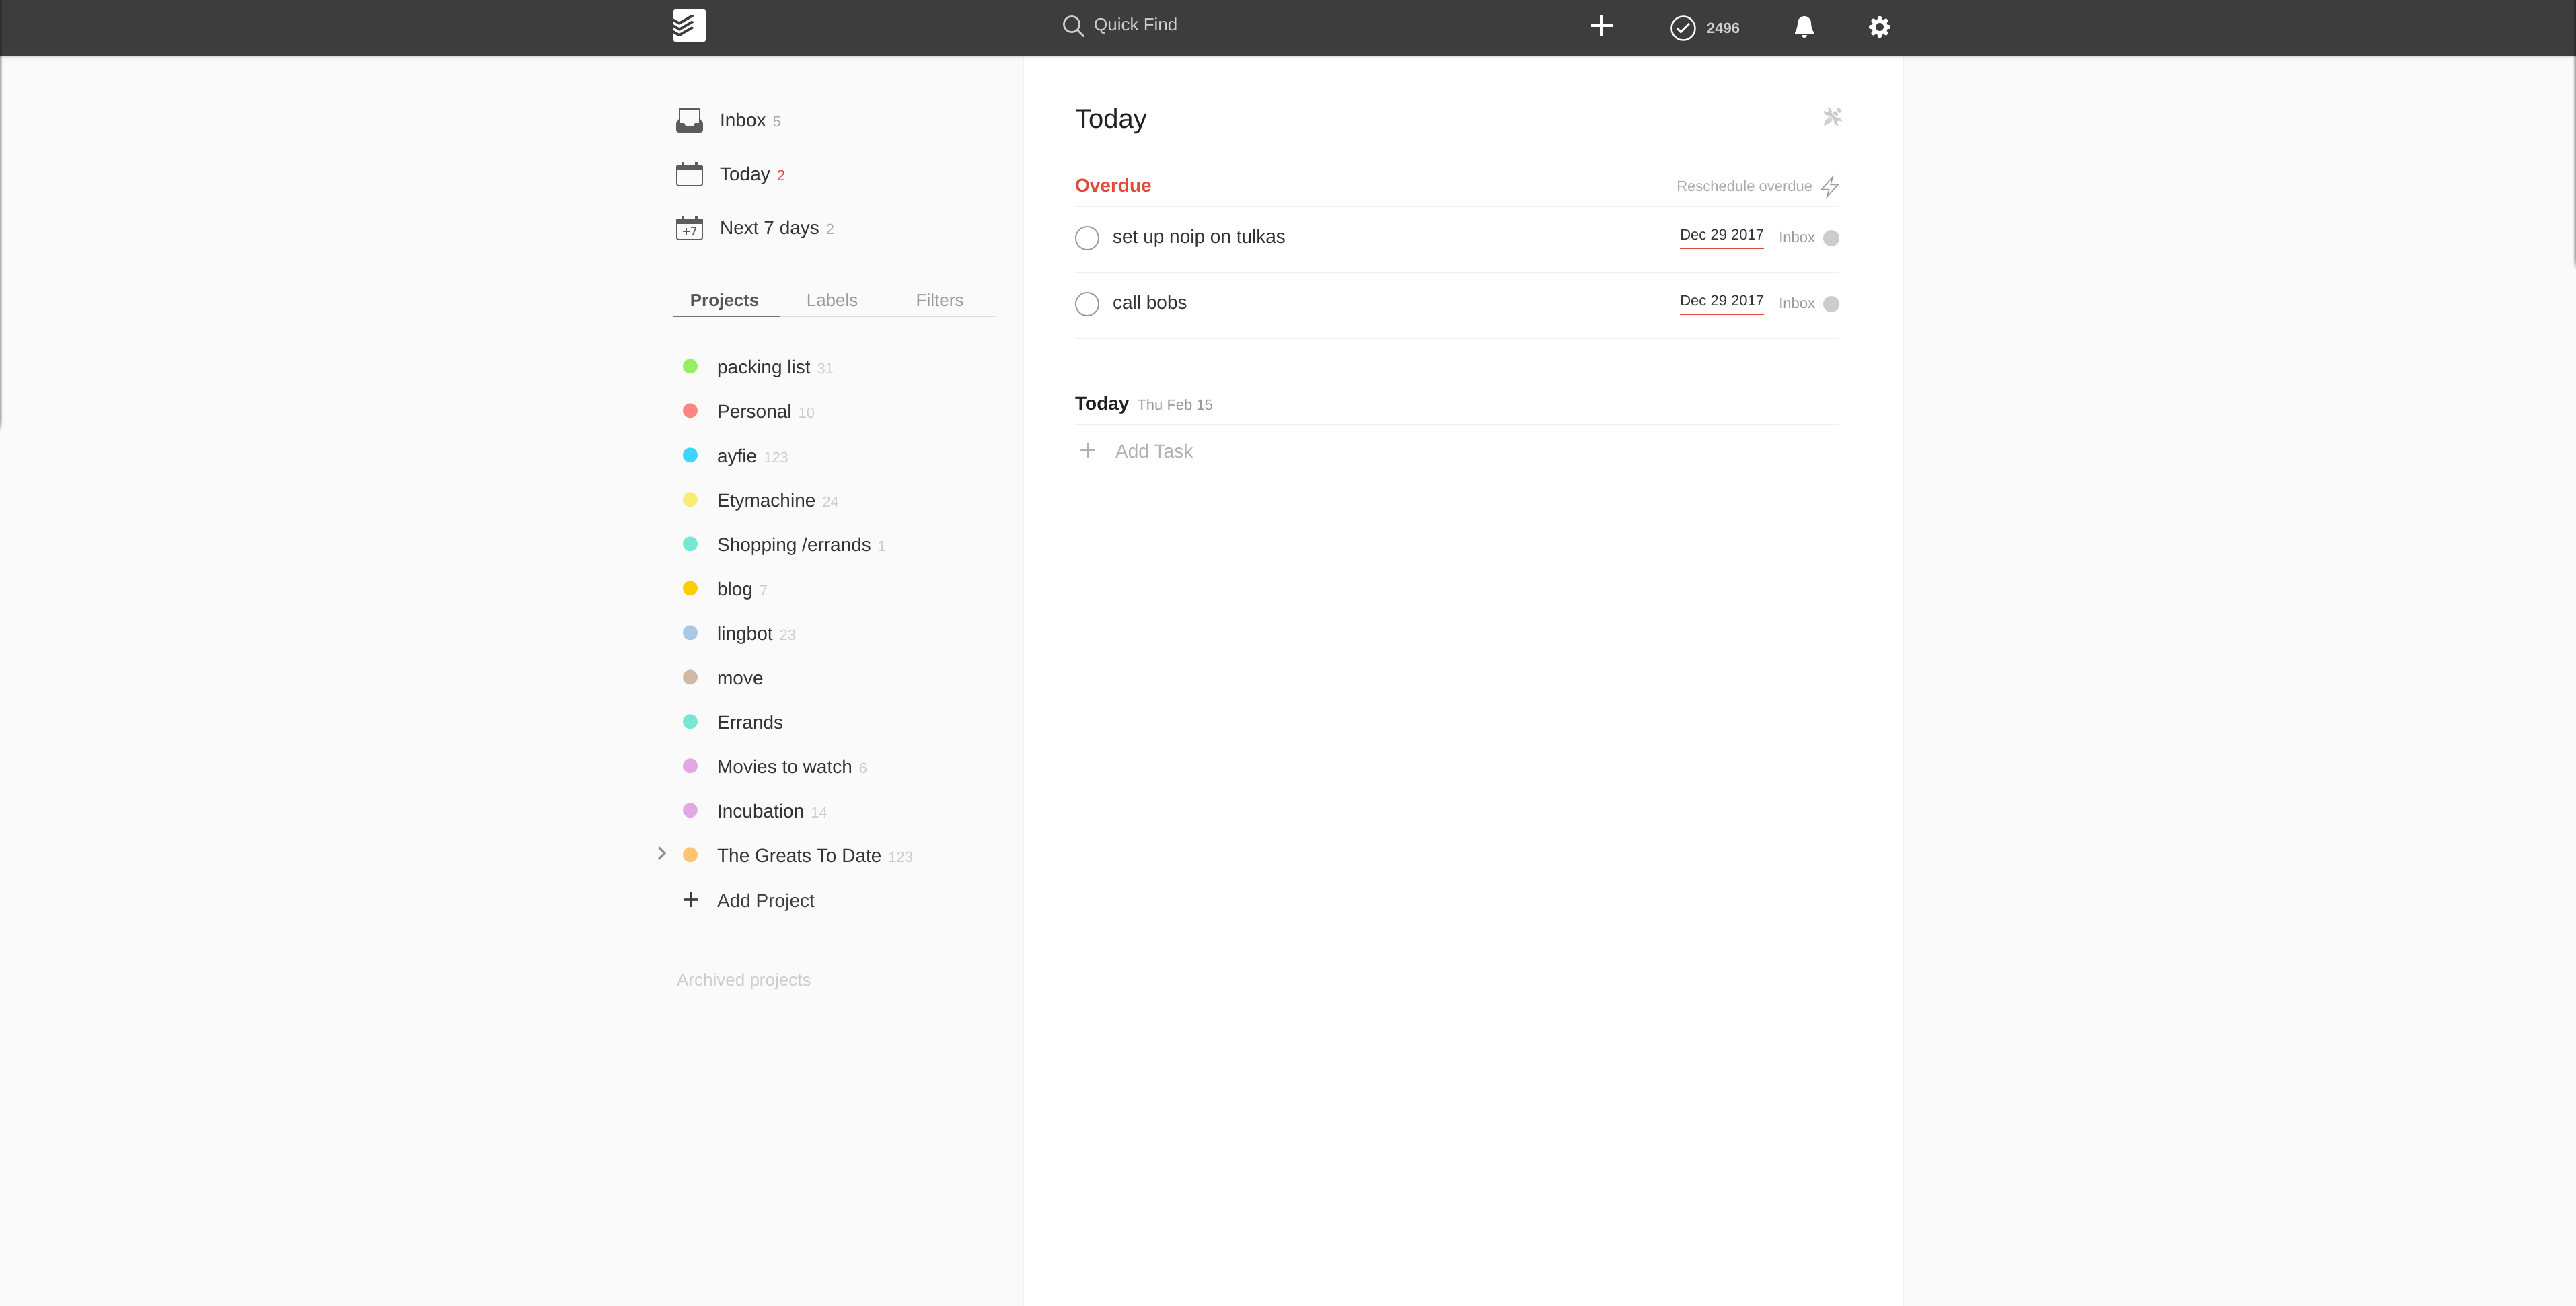
\includegraphics[width=12cm]{figs/todoist.png}}

\end{frame}

\begin{frame}[c]{Apps: Trello}

\centerline{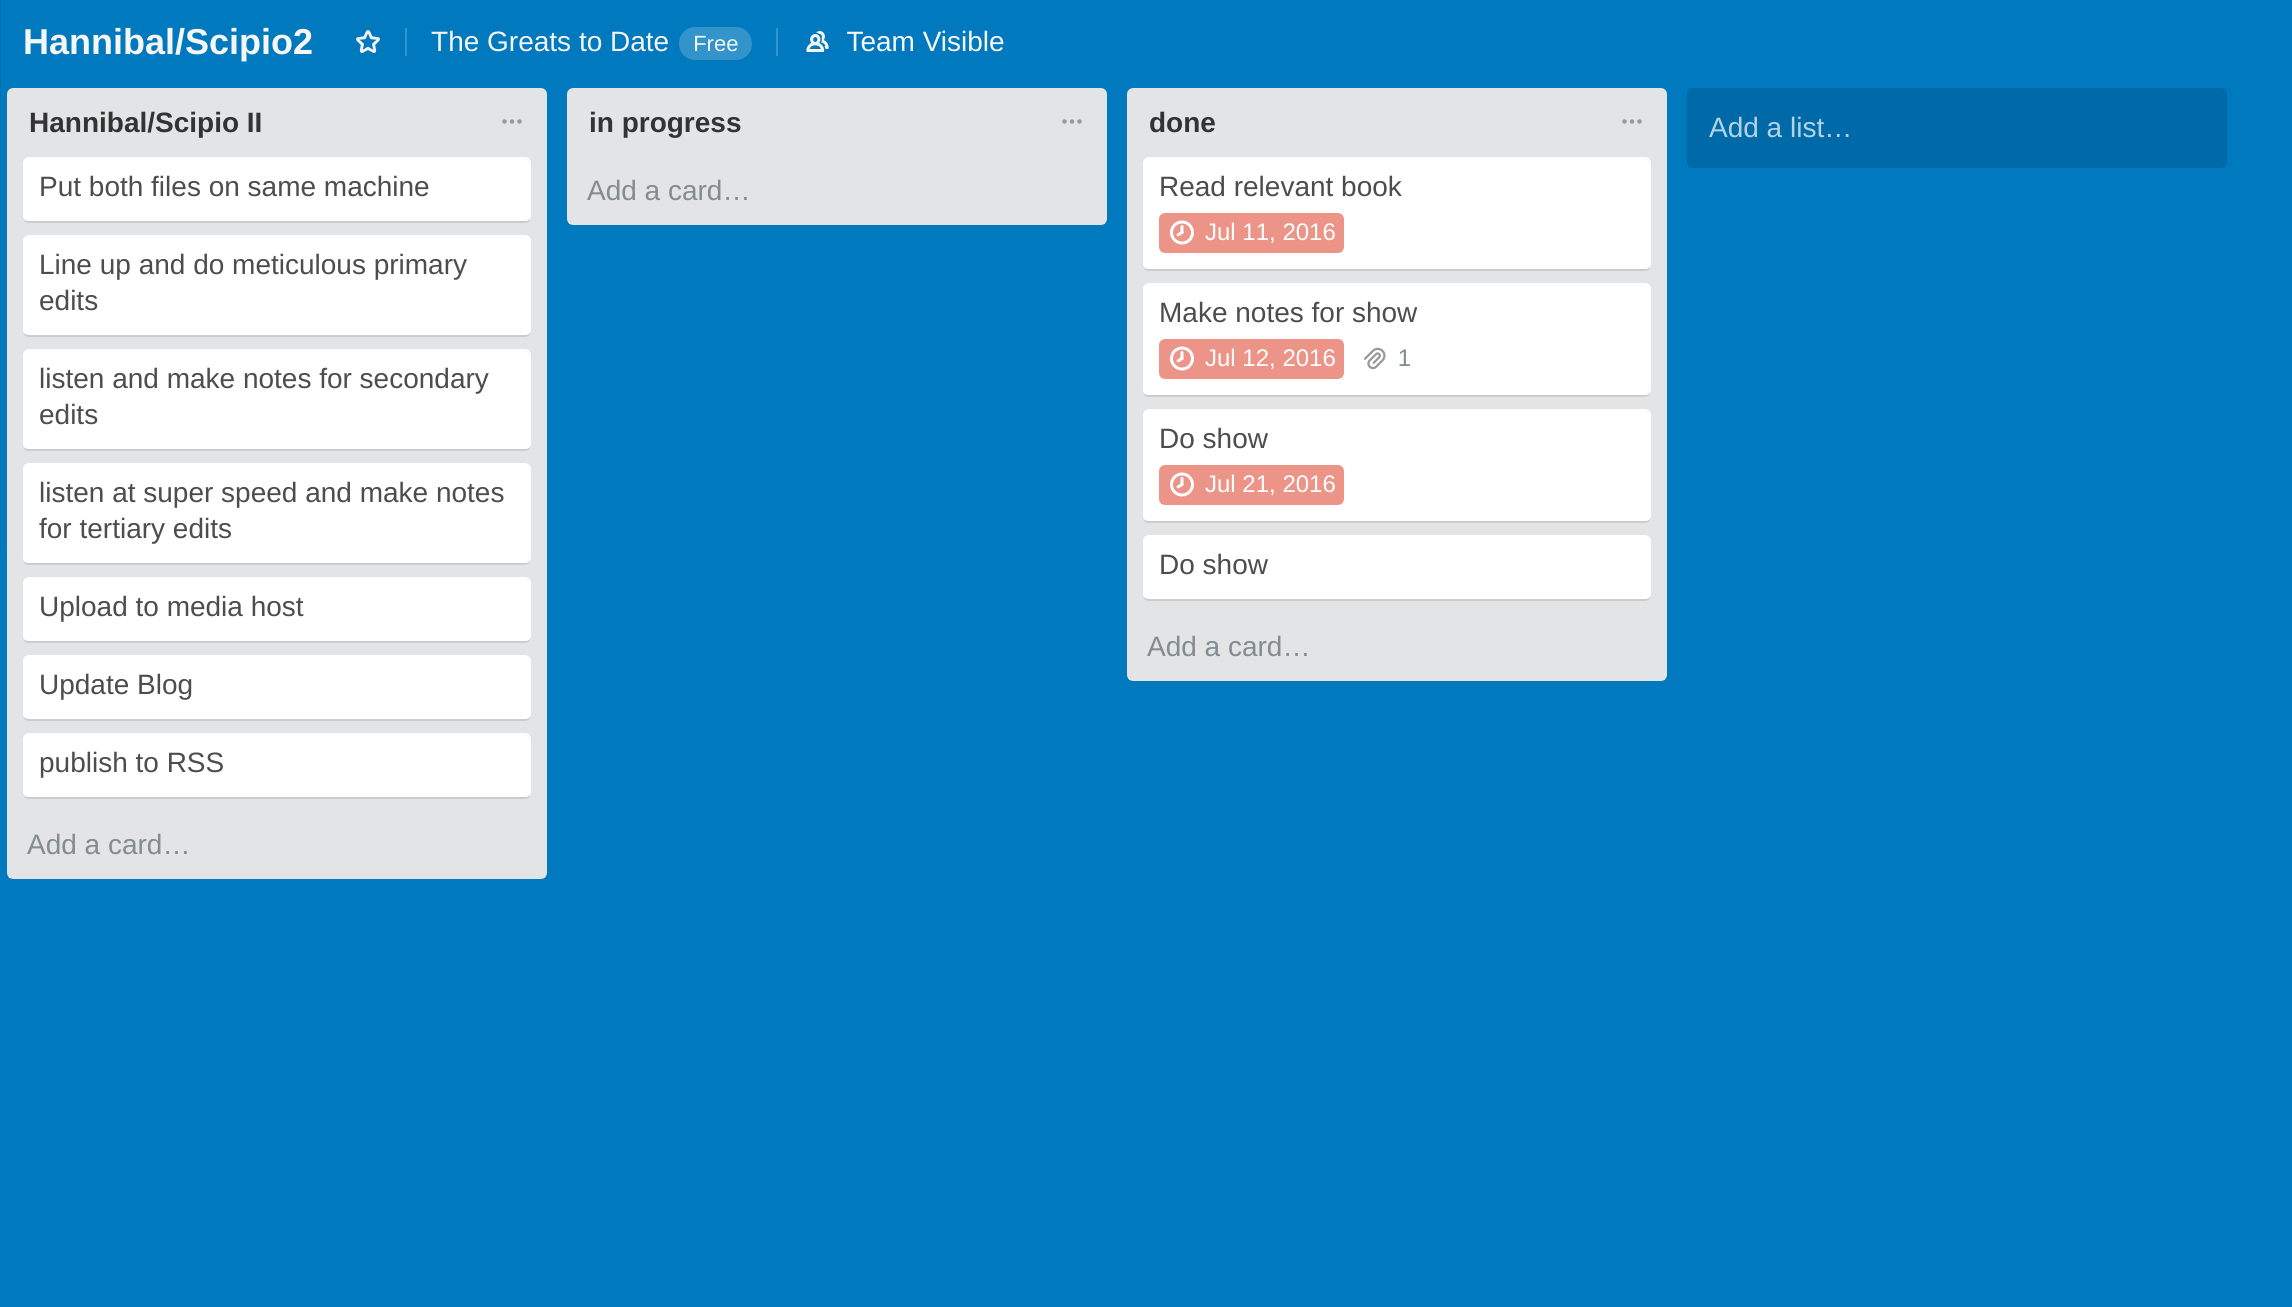
\includegraphics[width=12cm]{figs/trello.png}}

\end{frame}

\begin{frame}[c]{Apps: todo.txt}

\centerline{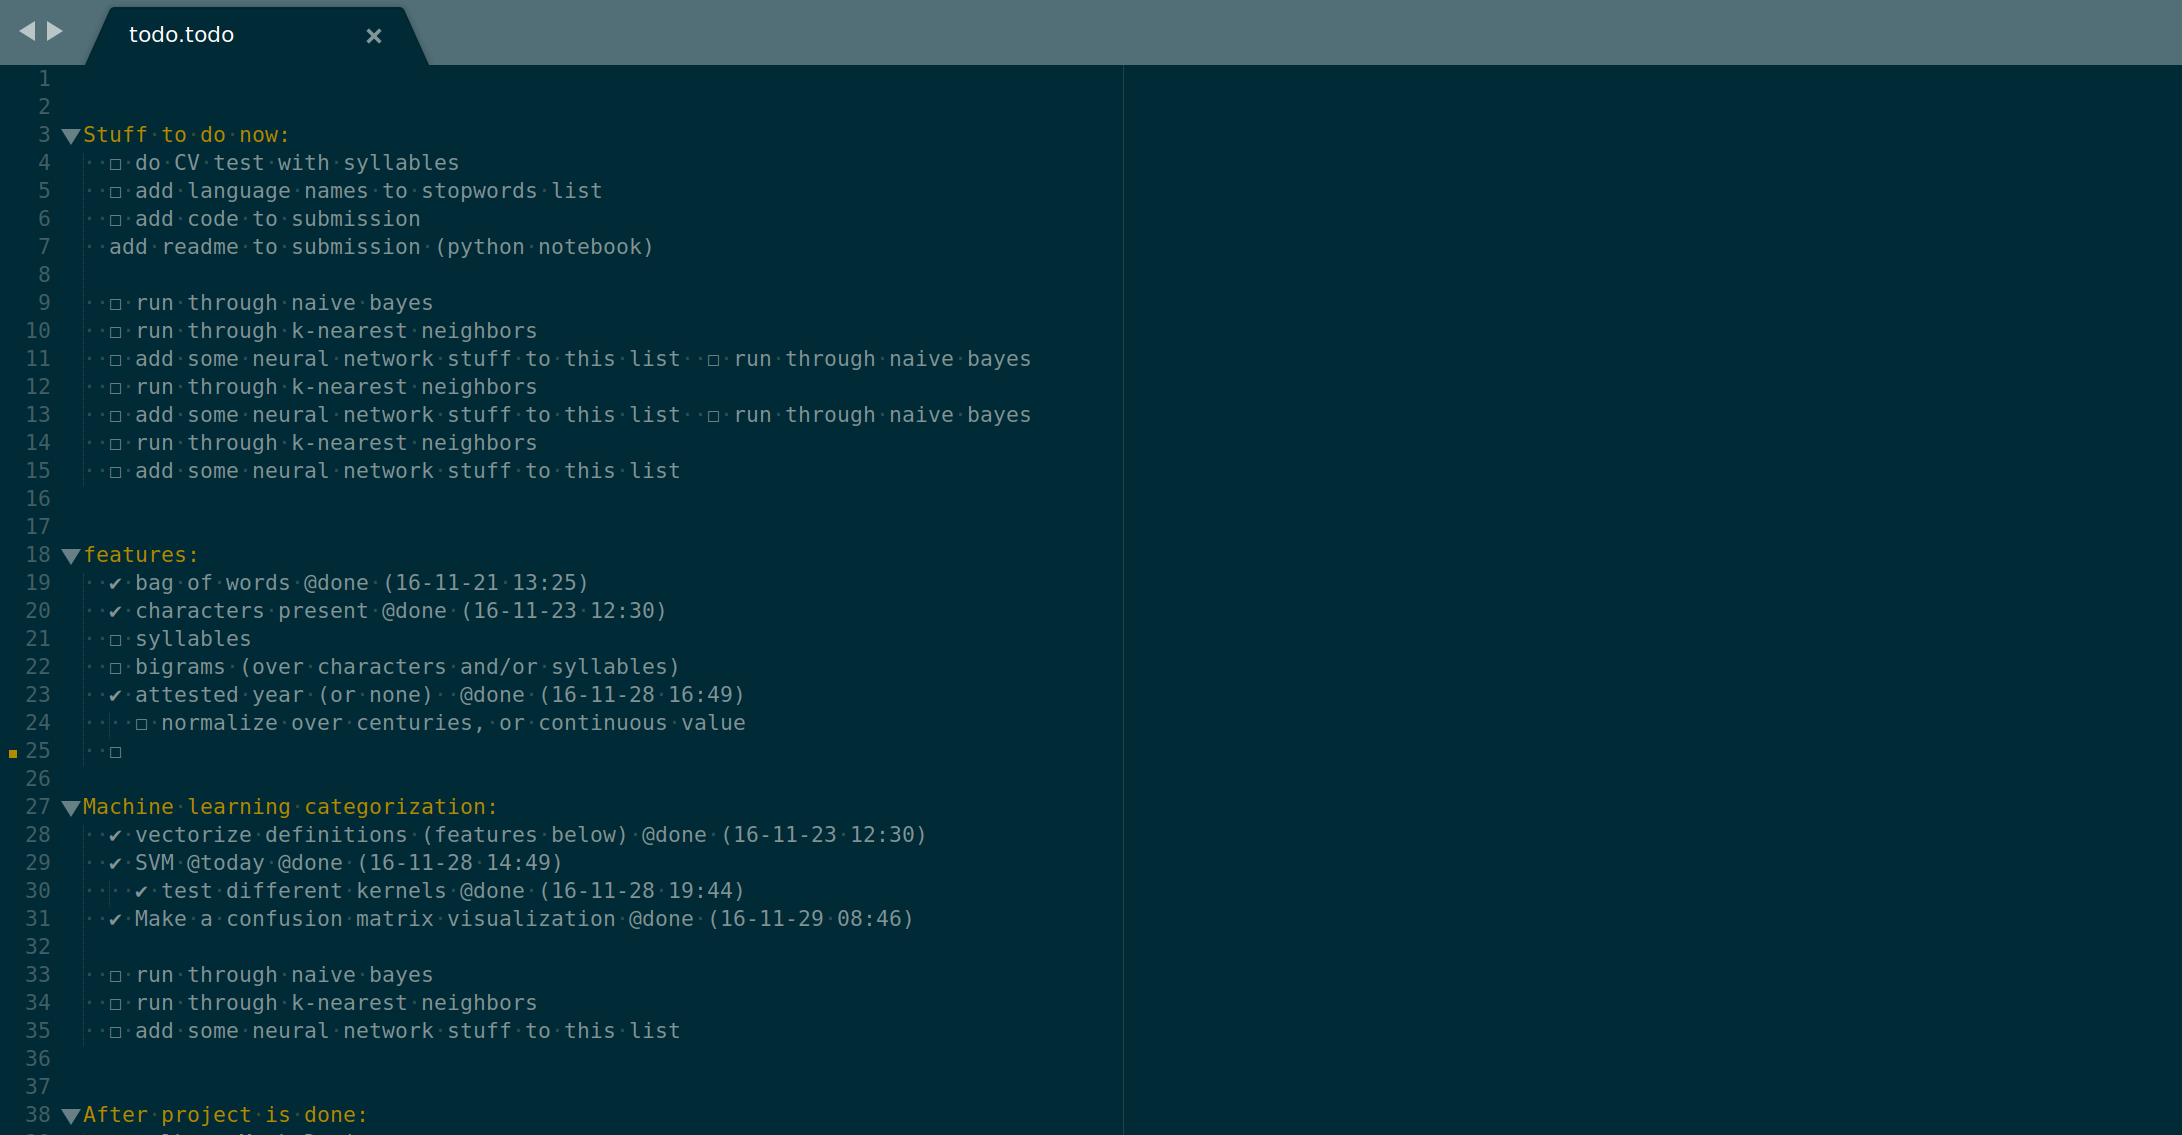
\includegraphics[width=12cm]{figs/todotxt.png}}

\end{frame}

\begin{frame}[c]{Apps: Bulletjournal}

\centerline{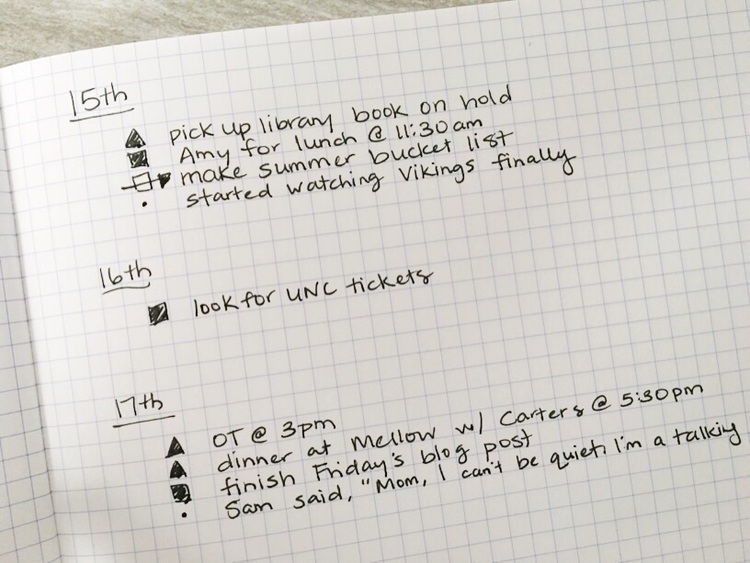
\includegraphics[width=12cm]{figs/bulletjournal.jpeg}}

\end{frame}

\begin{frame}[c]\frametitle{Advanced: Time tracking}

Not essential, but if you already have a good system for keeping track of your tasks.

\centerline{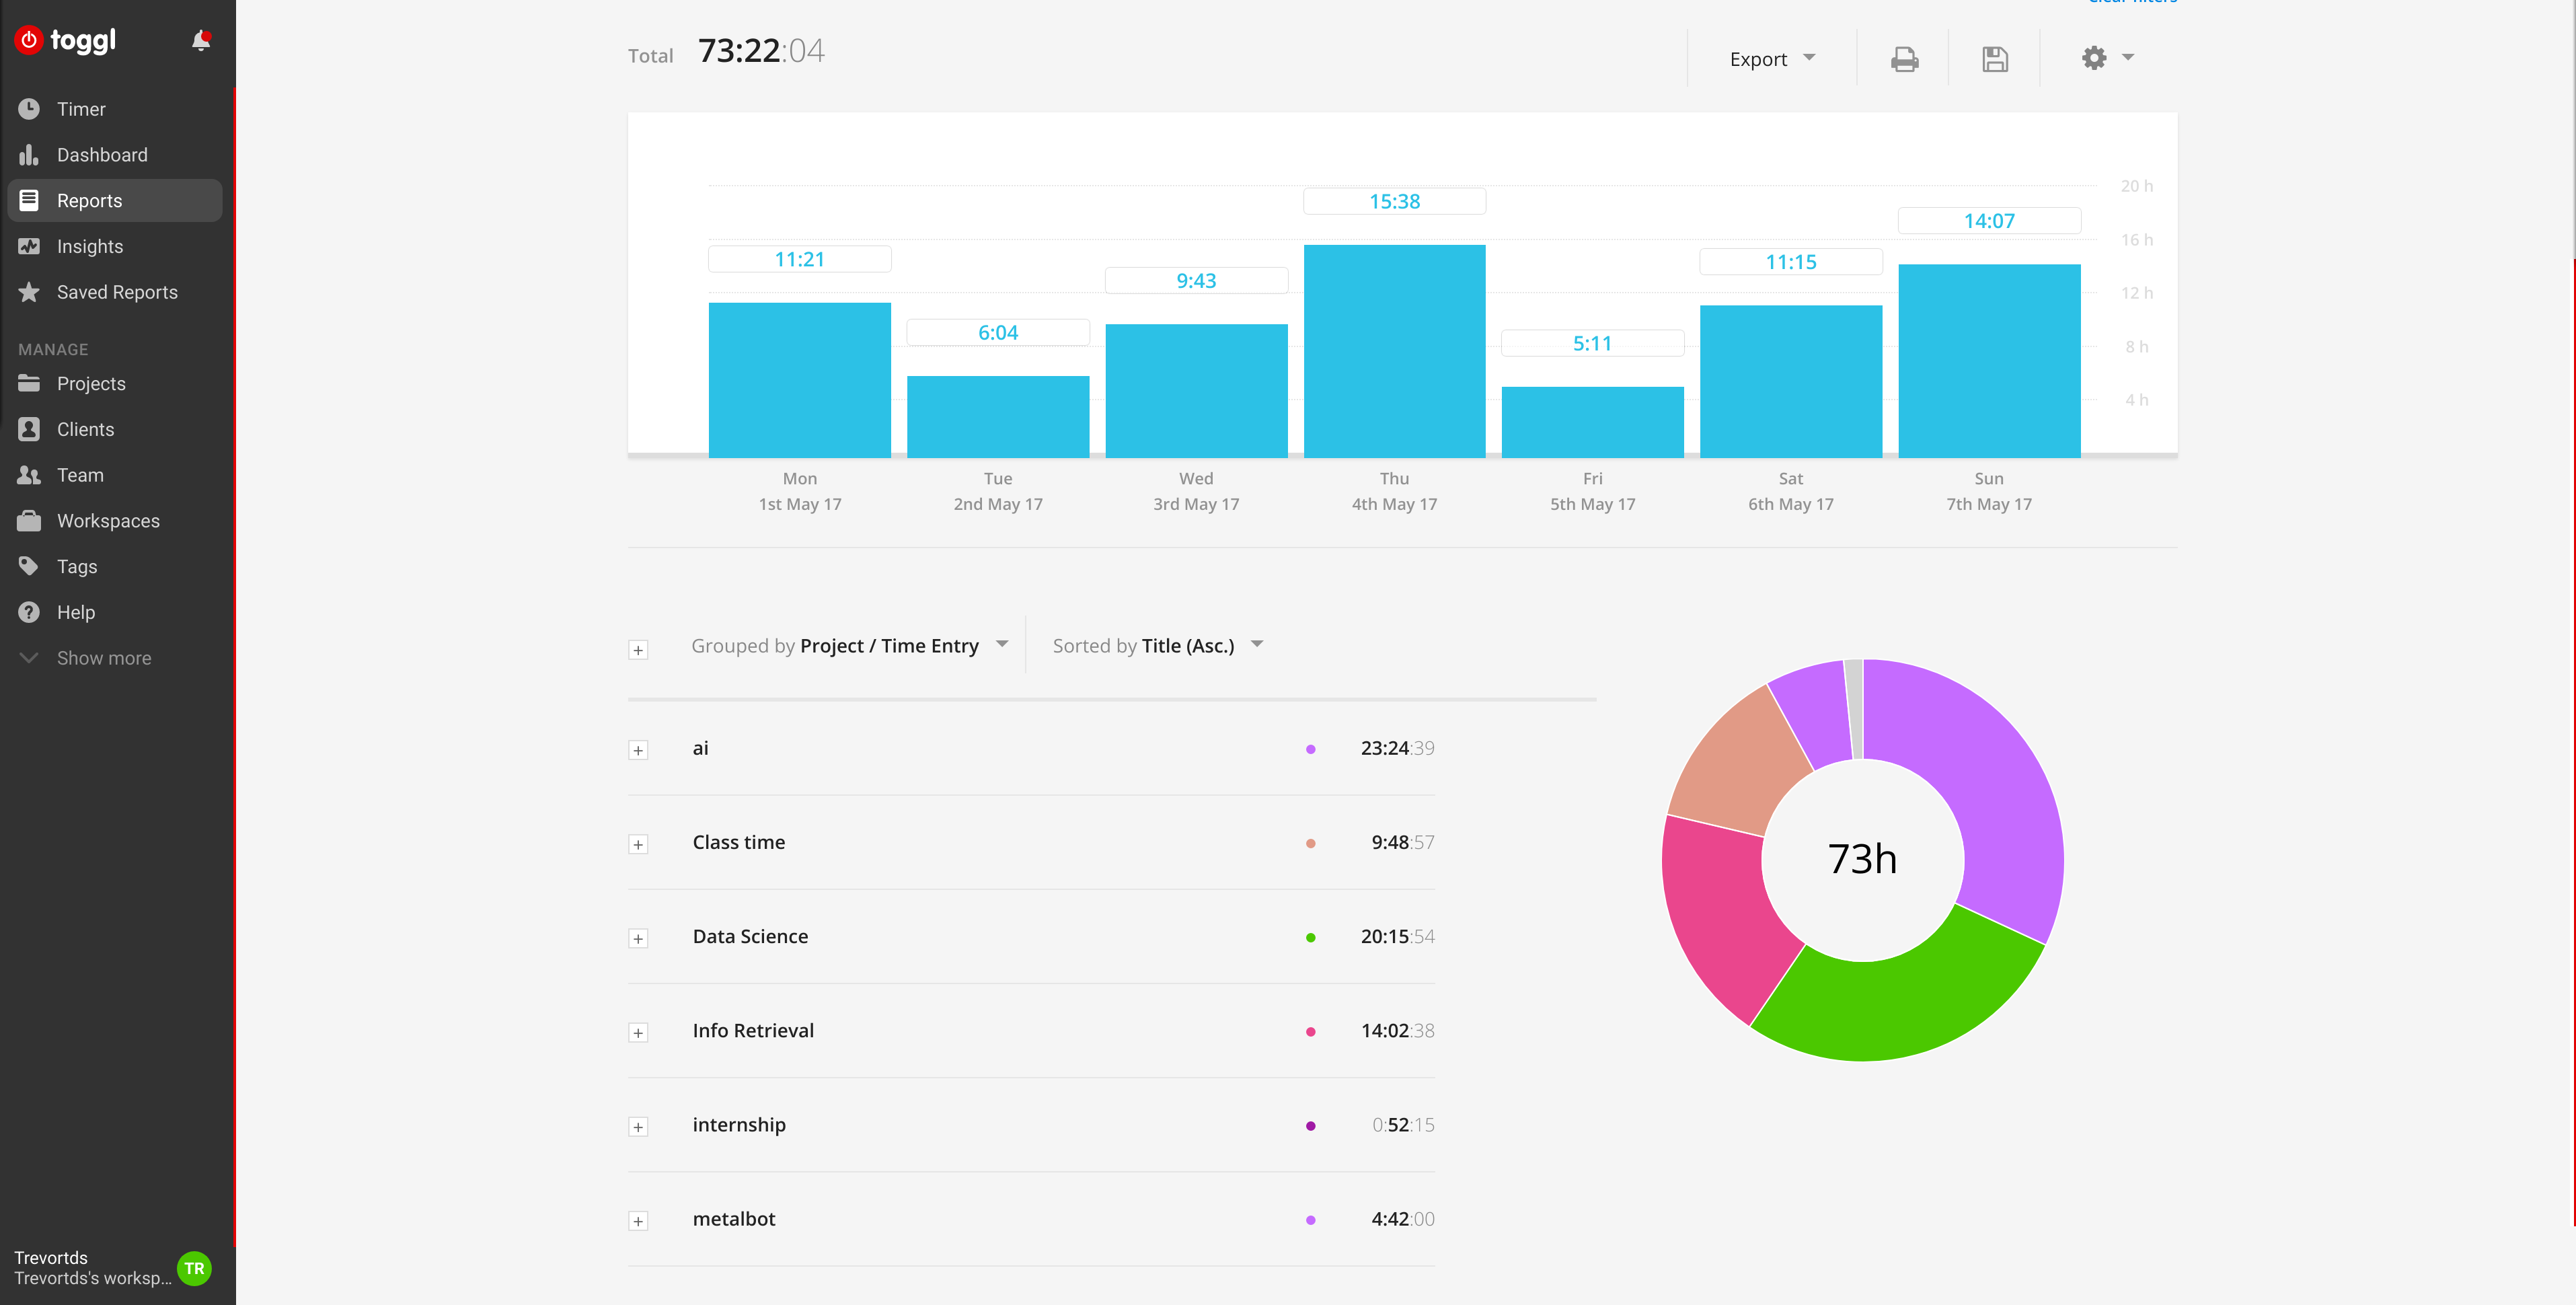
\includegraphics[width=10cm]{figs/toggl.png}}

\end{frame}

\begin{frame}[c]\frametitle{Super-Advanced: Automation}

Many of the aforementioned apps have APIs that can be manipulated manually, or through Zapier

\centerline{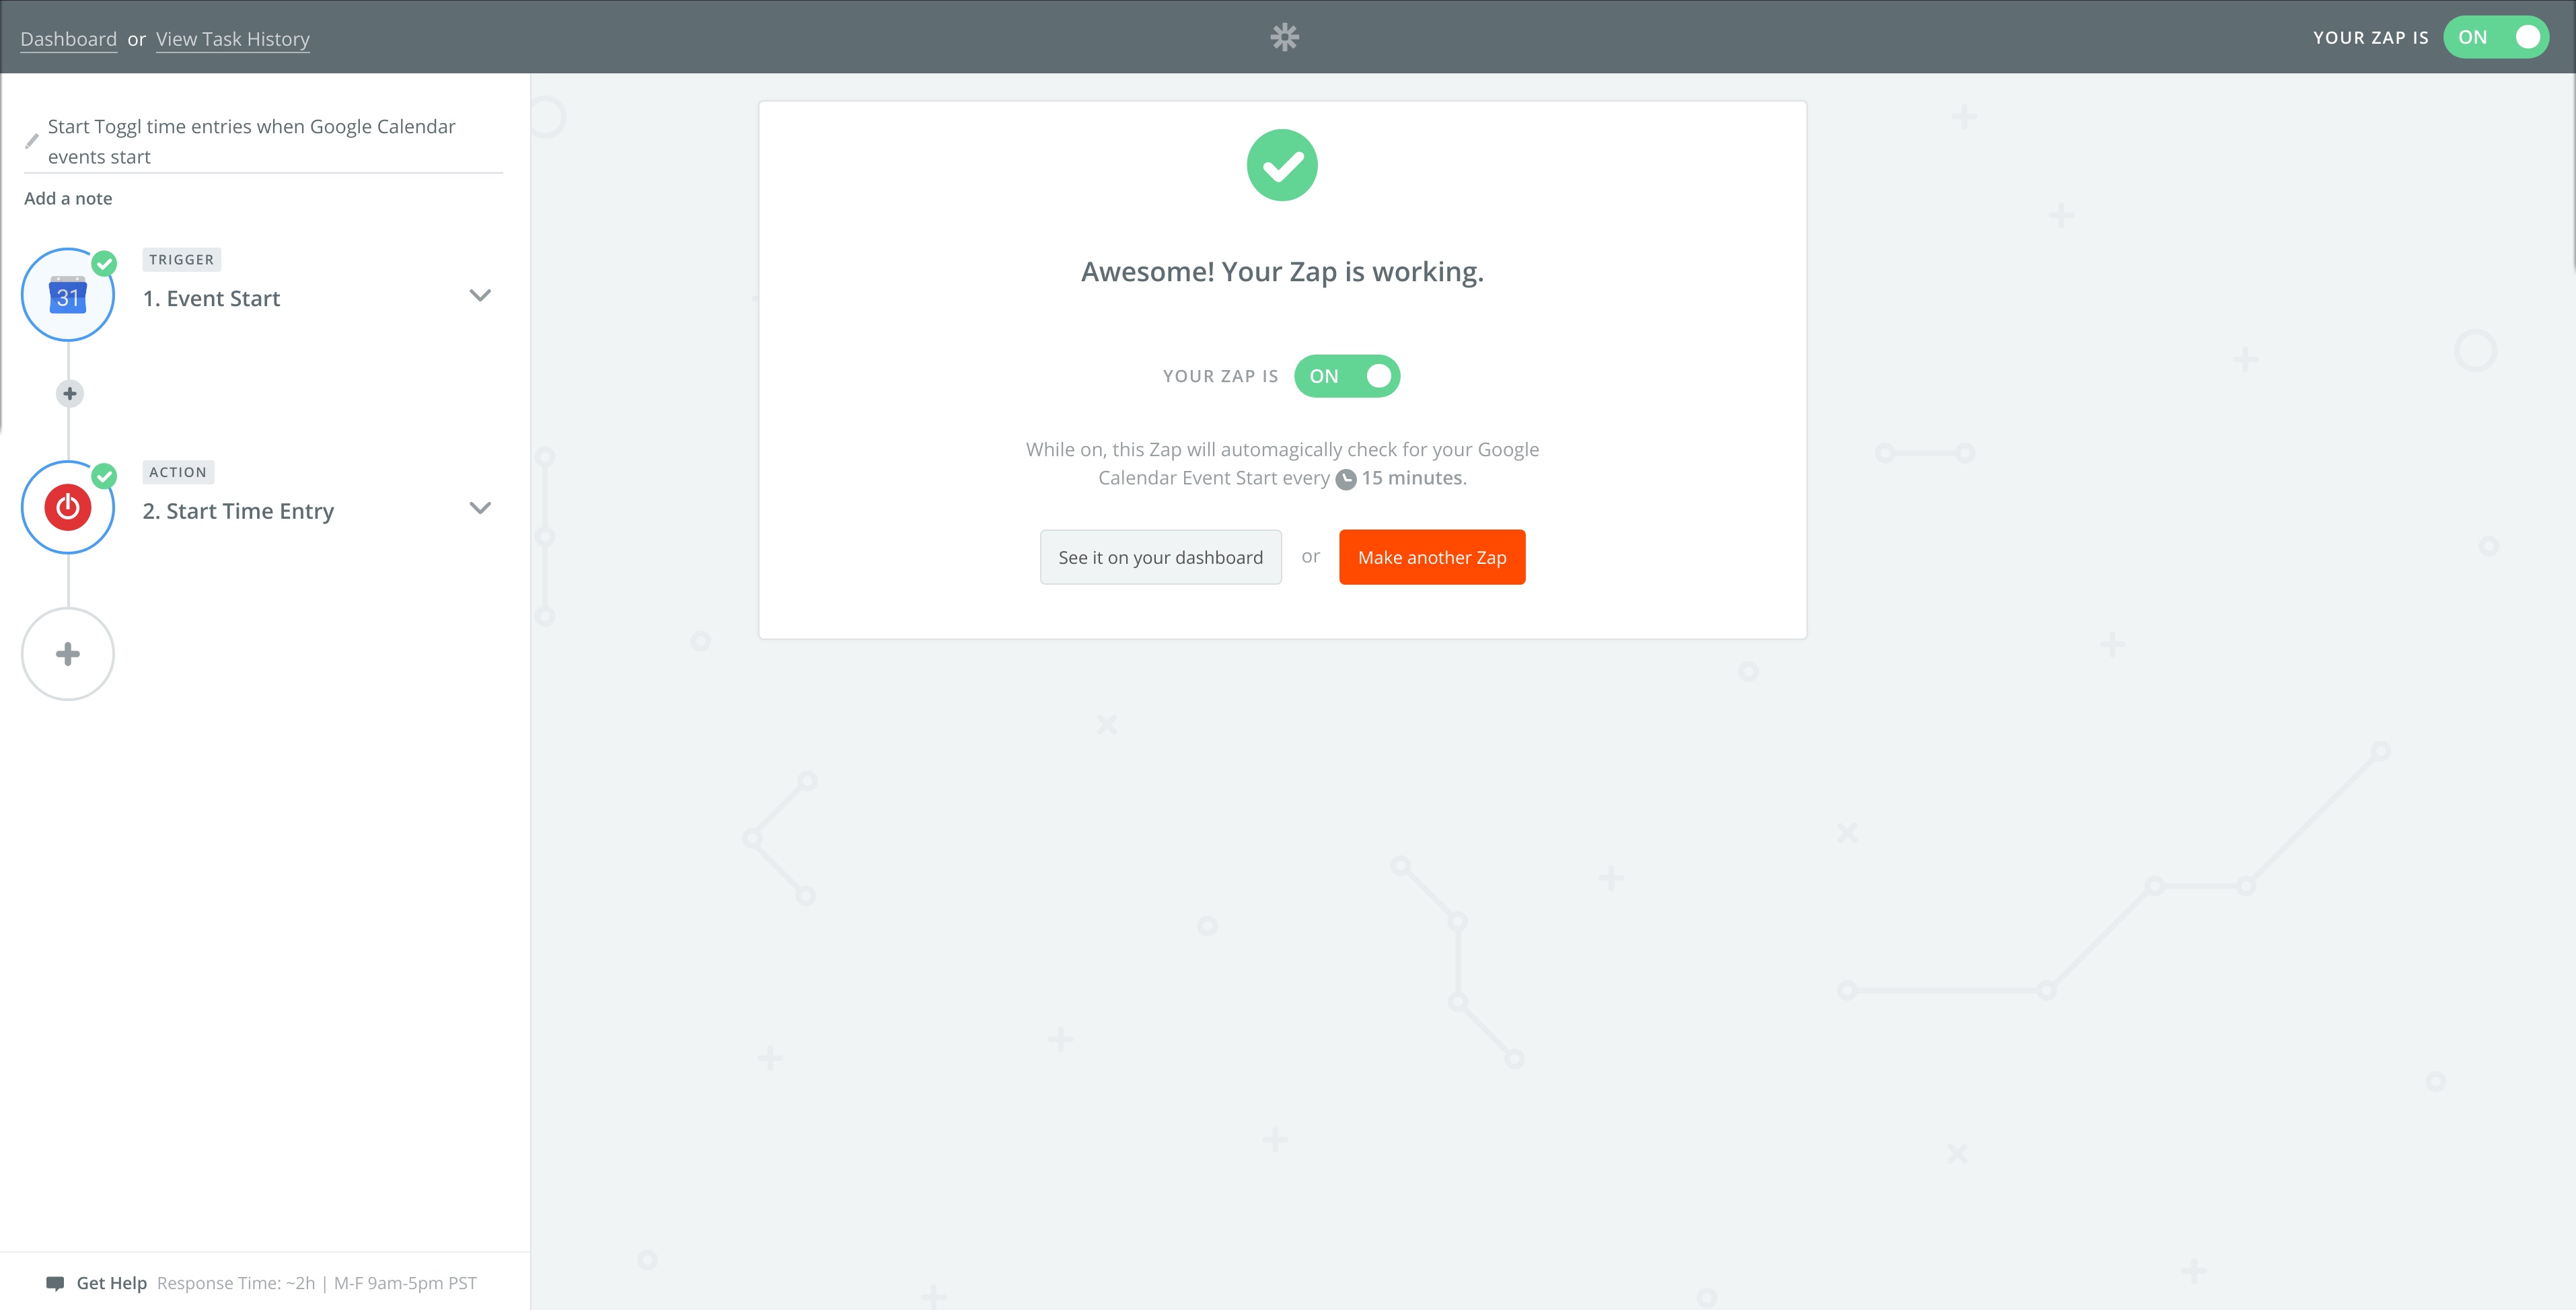
\includegraphics[width=10cm]{zapier.png}}

\end{frame}

\section{Docker, containerization, packaging | Git/Git-flow}

\begin{frame}[c]\frametitle{Be aware of: Docker, containerization, packaging}



\end{frame}

\begin{frame}[c]\frametitle{Maybe consider: yaml for configuration}



\end{frame}


\begin{frame}[c]\frametitle{Do it now: Git - not just for collaboration!}



\end{frame}


\section{Continuous Integration | Testing}

\begin{frame}[c]\frametitle{Be aware of: Continuous Integration}



\end{frame}


\begin{frame}[c]\frametitle{Do it now: Testing}



\end{frame}




\section{Cluster computing | Functional programming}

\begin{frame}[c]\frametitle{Be aware of: Cluster computing}



\end{frame}


\begin{frame}[c]\frametitle{Do it now: Functional programming}



\end{frame}

\appendix




\end{document}
